\begin{center}
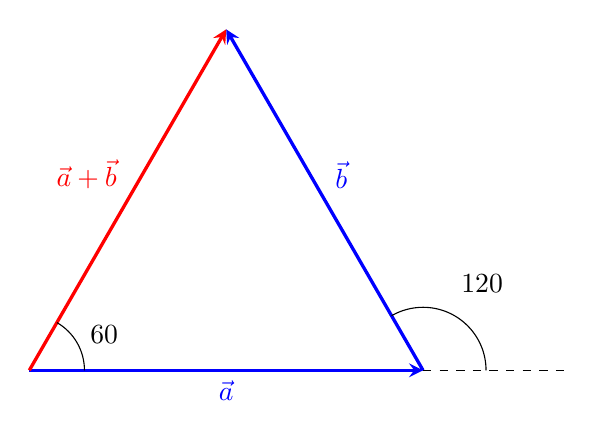
\begin{tikzpicture}[>=stealth]
 \draw[->, very thick, blue] (0,0) -- (5,0) node[midway, below] {$\vec a$};
 \draw[->, very thick, blue] (5,0) -- (2.5,4.33) node[midway, above right] {$\vec b$};
 \draw[->, very thick, red] (0,0) -- (2.5,4.33) node[midway, above left] {$\vec a+\vec b$};
 \draw[dashed] (5,0) -- (6.8,0);
 \draw (5.8,0) arc (0:120:0.8);
 \node at (5.75,1.1) {$\ang{120}$};
 \draw (0.7,0) arc (0:60:0.7);
 \node at (0.95,0.45) {$\ang{60}$};
\end{tikzpicture}
\end{center}

Setzt man die beiden Vektoren $\vec a$ und $\vec b$ aneinander, so bilden $\vec a$, $\vec b$ und die Summe $\vec a + \vec b$ ein Dreieck. Sind alle drei gleich lang, ist das Dreieck gleichseitig und alle Innenwinkel betragen $\ang{60}$.

Das ist genau dann der Fall, wenn die beiden Vektoren einen Winkel von $\result{\ang{120}}$ einschliessen (Winkel zwischen den Richtungen von $\vec a$ und $\vec b$, wenn man sie am gleichen Punkt anträgt).
